\chapter{Introduction to Adaptivity Analysis}
\label{introduction}



%%%% Benifit of reasoning about 
\section{Motivation of Reasoning about Adaptivity}
% 
Consider a dataset $X$ consisting of $n$ independent samples from some unknown population $\dist$.  How can we ensure that the conclusions drawn from $X$ \emph{generalize} to the population $\dist$?  Despite decades of research in statistics and machine learning on methods for ensuring generalization, there is an increased recognition that many scientific findings generalize poorly (e.g. 
\cite{Ioannidis05,GelmanL13}
).  While there are many reasons a conclusion might fail to generalize, one that is receiving increasing attention is \emph{adaptivity}, which occurs when the choice of method for analyzing the dataset depends on previous interactions with the same dataset~\cite{GelmanL13}.

 Adaptivity can arise from many common practices, such as exploratory data analysis, using the same data set for feature selection and regression, and the re-use of datasets across research projects.  Unfortunately, adaptivity invalidates traditional methods for ensuring generalization and statistical validity, which assume that the method is selected independently of the data. The misinterpretation of adaptively selected results has even been blamed for a ``statistical crisis'' in empirical science~\cite{GelmanL13}.
%  ~\cite{GelmanL13}.

\begin{figure}
    \centering
    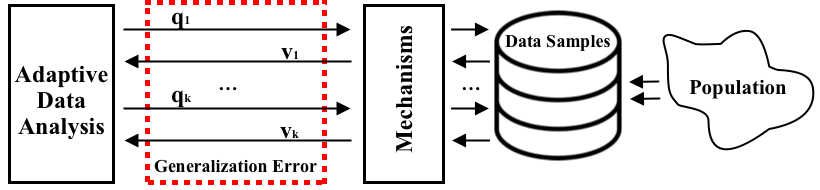
\includegraphics[width=0.7\columnwidth]{figures/data_analysis_model.png}
    \caption{Overview of our Adaptive Data Analysis model. We have a population that we are interested in studying, and a dataset containing individual samples from this population. The adaptive data analysis we are interested in running has access to the dataset through queries of some pre-determined family (e.g., statistical or linear queries) mediated by a mechanism. This mechanism uses randomization to reduce the generalization error of the queries issued to the data.}
    \label{fig:adaptivity-model-overview}
\vspace{-0.5cm}
\end{figure}

A line of work initiated by \citet{DworkFHPRR15}, \citet{HardtU14} posed the question: Can we design \emph{general-purpose} methods that ensure generalization in the presence of adaptivity, together with guarantees on their accuracy?  The idea that has emerged in these works is to use randomization to help ensure generalization. Specifically, these works have proposed to mediate the access of an adaptive data analysis to the data by means of queries from some pre-determined family (we will consider here a specific family of queries often called "statistical" or "linear" queries) that are sent to a  \emph{mechanism} which uses some randomized process to guarantee that the result of the query does not depend too much on the specific
sampled dataset. This guarantees that the result of the queries generalizes well. This approach is described in Figure~\ref{fig:adaptivity-model-overview}.  
This line of work has identified many new algorithmic techniques for ensuring generalization in adaptive data analysis, leading to algorithms with greater statistical power than all previous approaches. Common methods proposed by these works include, the addition of noise to the result of a query, data splitting, etc. Moreover, these works have also identified problematic strategies for adaptive analysis, showing limitations on the statistical power one can hope to achieve. Subsequent works have then further extended the methods and techniques in this approach and further extended the theoretical underpinning of this approach, e.g.~\cite{dwork2015reusable,dwork2015generalization,BassilyNSSSU16,UllmanSNSS18,FeldmanS17,jung2019new,SteinkeZ20,RogersRSSTW20}.
%

A key development in this line of work is that the best method for ensuring generalization in an adaptive data analysis depends to a large extent on the number of \emph{rounds of adaptivity}, the depth of the chain of queries. As an informal example, the program $x \leftarrow q_1(D);y \leftarrow q_2(D,x);z \leftarrow q_3(D,y)$ has three rounds of adaptivity, since $q_2$  depends on $D$ not only directly because it is one of its input but also via the result of $q_1$, which is also run on $D$, and similarly,  $q_3$ depends on $D$ directly but also via the result of $q_2$, which in turn depends on the result of $q_1$. The works we discussed above showed that, not only does the analysis of the generalization error depend on the number of rounds, but knowing the number of rounds actually allows one to choose methods that lead to the smallest possible generalization error - we will discuss this further in Section~\ref{sec:overview}. 

% \mg{Check the following - also the plots need to be on the same scale!}
For example, these works showed that when an adaptive data analysis uses a large number of rounds of adaptivity then a low generalization error can be achieved by mechanism of 
adding to the result of each query Gaussian noise scaled to the number of rounds. When instead  an adaptive data analysis uses a small number of rounds of adaptivity then a low generalization error can be achieved by using more specialized methods, such as data splitting mechanism or the reusable holdout technique from~\citet{DworkFHPRR15}.
To better understand this idea, we show in Figure~\ref{fig:generalization_errors} two experiments showcasing these situations. More precisely, in Figure~\ref{fig:generalization_errors}(a) we show the results of a specific analysis\footnote{We will use formally a program implementing this analysis (Figure~\ref{fig:overview-example}) as a running example in the rest of the paper.} with two rounds of adaptivity. This analysis can be seen as a classifier which first runs 500 non-adaptive queries on the first 500 attributes of the data, looking for correlations between the attributes and a label, and then runs one last query which depends on all these correlations. Without any mechanism the generalization error is pretty large, and the lower generalization error is achieved when the data-splitting method is used. 
In Figure~\ref{fig:generalization_errors}(b), we show the results of a specific analysis\footnote{We will present this analysis formally in Section~\ref{sec:examples}.} with four hundreds rounds of adaptivity. This analysis can be seen as a classifier which at each step runs an adaptive query based on the result of the previous ones. Again, without any mechanism the generalization error is pretty large, and the lower generalization error is achieved when the Gaussian noise is used. 

% As an example shown in Figure~\ref{fig:generalization_errors} presenting the experimental results of two adaptive data analysis with varied rounds of apdaptivity (2 in Figure~\ref{fig:generalization_errors}(a) and 500 in Figure~\ref{fig:generalization_errors}(b) ).  When a study includes queries with a large number of rounds of adaptivity, in Figure~\ref{fig:generalization_errors}(b), then a low generalization error can be achieved by adding Gaussian noise scaled to the number of rounds to the result of each query than data splitting.
% When instead a study includes queries with a low number of rounds of adaptivity as shown in Figure~\ref{fig:generalization_errors}(a), then it is easy to find that a low generalization error can be achieved by using more specialized methods, such as data splitting or the reusable holdout technique from~\citet{DworkFHPRR15}. 

% \jl{
% The Figure~\ref{fig:generalization_errors} shows an example illustrating the impact of adaptivity in the choice of mechanism to control the generalization error. 
% The x axis 
% % is Queries in this Data analysis sent to Server in each step of the data analysis,
% represents every query request in data analysis algorithm and
% % The y axis is Generalization Error of analysis result computed from every query.
% y axis for the empirical generalization error of 
% % analysis result computed from every query
% each query.
% There are three lines in Figure~\ref{fig:generalization_errors}(a) and (b),
% each 
% the green line represents the the empirical generalization error without using any mechanisms,
% the red on using the Gaussian mechanism and the blue one with the data-splitting mehcanism.
% % under a mechanism.
% By choosing different mechanisms, the generalization error is reduced in different degree in two data analysis strategy having different adaptivity rounds.
% % \\
% In Figure~\ref{fig:generalization_errors}(a), the data analysis algorithm
% has $k = 500$ non-adaptive queries but only $r = 2$ rounds 
% of adaptivity.
% % By choosing different mechanisms, the generalization error is reduced in different degree.
% It is obvious that we got better generalization results by choosing the data splitting mechanism than Gaussian mechanism.
% % \\
% However, in figure~\ref{fig:generalization_errors}(b), where the data analysis 
% has $k = 500$ queries in total as well as $r= 500$ rounds of adaptivity.
% % \\
% The generalization error is increasing as the query increasing, i.e., as the adaptivity 
% accumulating.
% In this $500$ rounds adaptive data analysis, by choosing Gaussian mechanism, we got better generalization results than choosing the data splitting mechanism.
% }
{\small
\begin{figure}
\centering
\begin{subfigure}{.48\textwidth}
\begin{centering}
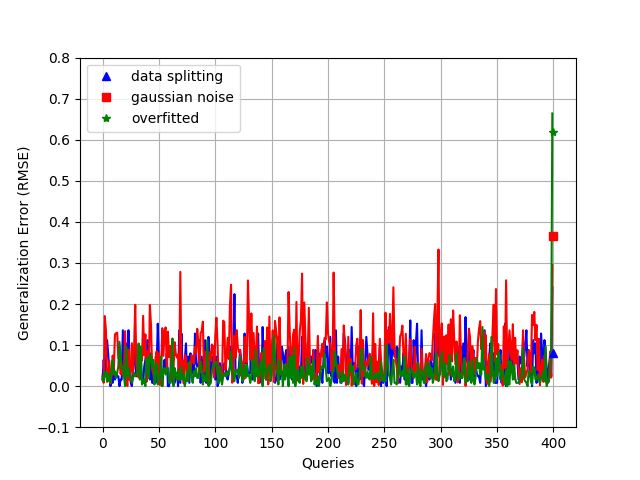
\includegraphics[width=0.9\textwidth]{figures/tworound.png}
\caption{}
\end{centering}
\end{subfigure}
%}
% \quad
% \centering
% \begin{subfigure}{.3\textwidth}
% \begin{centering}
% \includegraphics[width=0.9\textwidth]{tworound_datasplitting.png}
% \caption{}
% \end{centering}
% \end{subfigure}
%}
\quad
\begin{subfigure}{.48\textwidth}
\begin{centering}
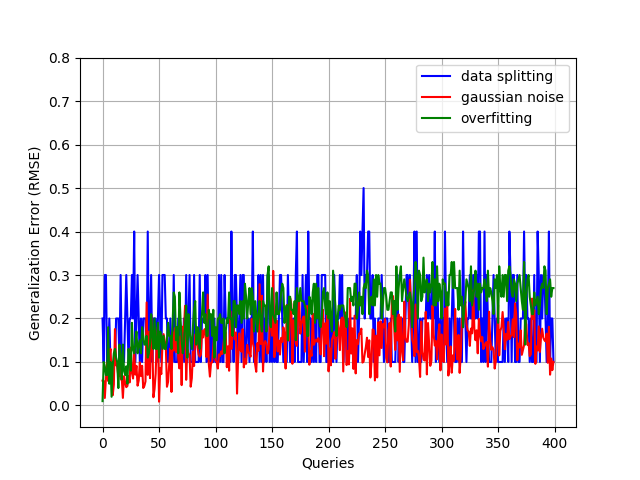
\includegraphics[width=0.9\textwidth]{figures/multipleround.png}
\caption{}
\end{centering}
\end{subfigure}
\vspace{-0.4cm}
 \caption{
 The generalization errors of two adaptive data analysis examples, under different choices of mechanisms.
 (a) Data analysis with adaptivity 2, 
 (b) Data analysis with adaptivity 400. 
}
\label{fig:generalization_errors}
\vspace{-0.5cm}
\end{figure}
}


%gap
This scenario motivates us to explore the design of program analysis techniques that can be used to estimate the number of \emph{rounds of adaptivity} that a program implementing a data analysis can perform. These techniques could be used to help a data analyst in the choice of the mechanism to use,
and they
could be ultimately be integrated into a tool for adaptive data analysis such as the \emph{Guess and Check} framework by~\citet{RogersRSSTW20}. 
%

The first problem we face is \emph{how to define formally} a model for adaptive data analysis which is general enough to support the methods we discussed above and would permit to formulate the notion of adaptivity these methods use. 
We take the approach of designing a programming framework for submitting queries to some \emph{mechanism} giving access to the data mediated by one of the techniques we mentioned before, e.g., adding Gaussian noise, randomly selecting a subset of the data, using the reusable holdout technique, etc. 
In this approach, a program models an \emph{analyst} asking a sequence of queries to the mechanism. The mechanism runs the queries on the data applying one of the methods discussed above and returns the result to the program. The program can then use this result to decide which query to run next. 
Overall, we are interested in controlling the generalization of the results of the queries which are returned by the mechanism, by means of the adaptivity. 

The second problem we face is \emph{how to define the adaptivity of a given program}.
Intuitively, a query $Q$ may depend on another query $P$, if there are two values that $P$ can return which affect in different ways the execution of $Q$. 
For example, as shown in \cite{dwork2015reusable}, and as we did in our example in Figure~\ref{fig:generalization_errors}(a), one can design a machine learning algorithm for constructing a classifier which first computes each feature's correlations with the label via a sequence of queries, and then constructs the classifier based on the correlation values. 
If one feature's correlation changes, the classifier depending on features is also affected.  
This notion of dependency builds on the execution trace as a \emph{causal history}. 
In particular, we are interested in the history or provenance of a query up until this is executed, we are not then concerned about how the result is used --- except for tracking whether the result of the query may further cause some other query. 
This is because we focus on the generalization error of queries and not their post-processing. % 
To formalize this intuition as a quantitative program property,
% we first consider all the possible evaluations of a programs  --- we do this by 
we use a trace semantics recording the execution history of programs on some given input --- and we create a dependency graph, where the dependency between different variables (query is also assigned to variable) is explicit and track which variable is associated with a query request. 
We then enrich this graph with weights describing the maximal number of times each variable is evaluated in a program evaluation starting with an initial state. The adaptivity is then defined as the length of the walk visiting most query-related variables on this graph. 

The third problem we face is \emph{how to estimate the adaptivity of a given program}. 
The adaptive data analysis model we consider and our definition of adaptivity suggest that for this task we can use a  program analysis that is based on some form of dependency analysis. This analysis needs to take into consideration:
1) the fact that, in general, a query $Q$ is not a monolithic block but rather it may depend, through the use of variables and values, on other parts of the program. 
Hence, it needs to consider some form of data flow analysis. 
2) the fact that, in general, the decision on whether to run a query or not may depend on some other value. Hence, 
 it needs to consider some form of control flow analysis.
3) the fact that. in general, we are not only interested in whether there is a dependency or not, but in the length of the chain of dependencies. 
Hence, it needs to consider some quantitative information about the program dependencies. % {A quick example is that : we store the result of query $Q_1$ in variable $x$ and use variable $y$ to record the result of query $Q_2$. We want to construct the third query $Q_3$ which relies on the value stored in $x$, let us say, $Q_3$ will ask for the sum of the first column of a table if $x$ is positive and the sum of the second column otherwise. In this situation, we need data flow analysis. On the other hand, if we need the value of $y$ to help us decide whether we should ask $Q_3$, for example, we ask the third query if $y$ is odd, and do not ask if $y$ is even. Naturally, to be able to handle this case, control flow analysis comes into play. Formally speaking,  }
To address these considerations and be able to estimate a sound upper bound on the adaptivity of a program, 
we develop a program analysis algorithm, named {\ADAPTSYSTEM}, which combines data flow and control flow analysis with reachability bound analysis~\cite{GulwaniZ10}. 
This new program analysis gives tighter bounds on the adaptivity of a program than the ones one would achieve by directly using the data and control flow analyses or the ones that one would achieve by directly using reachability bound analysis techniques alone.
%%%%% To reason about
\section{Methodology}
We use static analysis techniques to reason about the two main quantitative properties studied in this dissertation: 
the adaptivity of adaptive data analysis programs,
the reachability bound of while loop programs. 

\subsection{Abstract Interpretation}

\subsection{Dependency Graph}
Another quantitative property we study is the adaptivity of adaptive data analysis programs. 
{The adaptivity is defined to be the length of the longest chain of queries of the program in which one query may rely 
on its previous queries in the same chain. 
The adaptivity of a data analysis program is quite different from the relative cost of the two programs. To reason about cost, we can simply sum the costs of sub-programs to get the upper bound of the cost. However, the adaptivity of each sub-program of the target program does not help much in finding the adaptivity. To use a type and effect system to reason about adaptivity, this system should be able to express certain dependencies.
% Of course, we can sum them but then the result becomes imprecise. For this reason, we think the type and effect system is not the good direction to reason about the adaptivity of a data analysis program since it is tricky for the effect to carry information such as one query may depend on the other one. 
We expect adaptivity can also be reasoned about by type and effect systems but in this work, we choose to use a dependency graph to reason about adaptivity.}

{There are two challenges to reason about adaptivity: what will a formal definition of the adaptivity of a data analysis program look like, and how to reason about the adaptivity. 
In our work, the first challenge is solved by a query-based dependency graph generated along with the evaluation of the program. 
Our trace-based operational semantics can generate the trace which tracks the queries asked in the evaluation of the program. 
The query-based dependency graph is constructed based on the queries in the trace. Every node of the graph represents a unique query asked in the program, and the directed edge between two nodes, identifying one query (one node) may depend on the other one. 
The adaptivity is then formally defined as the length of the longest path in the query-based dependency graph.}
{The second challenge is how to estimate the adaptivity of a data analysis program we have just defined. 
In order to upper bound the length of the longest path in the query-based dependency graph, we want to find a path in a dependency graph as well such that the path contains all the queries in that longest path in the query-based dependency graph. 
We develop an algorithm to build a variable-based dependency graph, in which every node represents the unique variable that is assigned in one assignment statement of the program. 
The direct edge between two nodes reflects both the data dependency and control flow dependency between variables. Also, we add the unit weight to the node whose variable is associated with a query result. Then the upper bound on the adaptivity of the data analysis program is estimated by the weight of the path with the highest weights in the variable-based dependency graph.}

{To summarize, we use two dependency graphs for reasoning about the adaptivity of a data analysis program: 
one query-based dependency graph to define the adaptivity, and one weighted variable-based dependency graph to estimate an upper bound on the adaptivity. }

\section{Contributions}

Program analysis techniques are usually applied to study quantitative properties. In comparison to those related works, this dissertation has the following contributions.

\begin{enumerate}

\item We propose a formal definition of the adaptivity of adaptive data analysis programs and develop a graph-based program analysis algorithm that statically estimates the adaptivity.
\item reachability bound computing algorithm
% To the best of our knowledge, it is the first work that statically estimates adaptivity to help design adaptive data analysis algorithms.  
\end{enumerate}

\section{Dissertation Outline}
This dissertation includes two main parts. 
One reasons about the quantitative property (cost) of programs in the relational setting. Another one aims to use the quantitative property (adaptivity) of adaptive data programs indirectly, as an auxiliary component in data analysis research.

The rest of the dissertation is divided into $3$ parts. 
\begin{enumerate}
    \item Part (1) Chapter~\ref{ch:language}
    
    \item Part {2} Chapter~\ref{ch:dynamic}
    
    \item Part (3) Chapter~\ref{ch:static} shows the work on the program analysis algorithms to study the adaptivity of the adaptive data analysis program.    

Chapter~\ref{ch:adapt_intro} gives the introduction of adaptive data analysis in Section~\ref{sec:adapt-backgroung} and the challenges (Section~\ref{sec:adapt-challenges}) we face to obtain the adaptivity to control the generalization error of an adaptive data analysis program.

Chapter~\ref{ch:adapt-definition} presents the details of the loop language (Section~\ref{sec:adapt-loop-syntax}) we use to express data analysis programs, and shows the definition of adaptivity from a trace-based operational semantics in Section~\ref{sec:adapt-os}. 


Chapter~\ref{ch:adapt-algo} describes the program analysis algorithm {\ADAPTSYSTEM} that used to estimate the adaptivity of the data analysis programs (Section~\ref{sec:adapt-ve}, Section~\ref{sec:adapt-matrix}). 
The idea behind the algorithms (Section~\ref{sec:adapt-algo-ideas}) is to construct a data control dependency graph, and add weights to the graph. The adaptivity is estimated by the weight of the path with the highest weight.

Chapter~\ref{ch:adapt-example} presents some more interesting examples {\ADAPTSYSTEM} can analyse. 
It includes a variant of two round data analysis algorithm (Section~\ref{sec:adapt-example-tr-odd}), 
an adaptive multiple rounds data analysis algorithm (Section~\ref{sec:adapt-example-mr}) and an example showing the over-approximate of our approach (Section~\ref{sec:adapt-example-over}). 

Chapter~\ref{ch:adapt-relatedwork} discusses the related works from three perspectives: Static program analysis (Section~\ref{sec:adapt-rw-static}), dynamic program analysis (Section~\ref{sec:adapt-rw-dynamic}) and generalization in adaptive data analysis (Section~\ref{sec:adapt-rw-ge}).  
\item Part {4} ~ concludes the dissertation and discusses the future directions on studying the two quantitative properties: relative cost and adaptivity.
\item Part {5} ~gives the appendices. 
 The appendix~\ref{AppC} gives the proof of the lemmas of our framework in adaptive data analysis.    
\end{enumerate}



\section{Previous Published Material}
The contents of this dissertation are partly based on the work and writing in the following papers.

% The work of{\ADAPTSYSTEM} is still under preparation.


